单独的相互作用网络也是很有用的模型,但是,如果能跟其它信息整合在一起,则能回答更多的科学疑问。


Interaction networks are useful as stand-alone models. However, they are most
powerful for answering scientific questions when integrated with additional
information. Cytoscape allows the user to add arbitrary node, edge and network
information to Cytoscape as node/edge/network attributes. This could include,
for example, annotation data on a gene or confidence values in a
protein-protein interaction. These attributes can then be visualized in a
user-defined way by setting up a mapping from data attributes to visual
attributes (colors, shapes, and so on). The section on  visual styles discusses
this in greater detail. 

\subsubsection{Cytoscape~属性文件格式}

 Node and edge attribute files are simply formatted: a node attribute file
begins with the name of the attribute on the first line (note that it cannot
contain spaces). Each following line contains the name of the node, followed by
an equals sign and the value of that attribute. Numbers and text strings are
the most common attribute types. All values for a given attribute must have the
same type. For example: 

 \begin{verbatim}
FunctionalCategory
YAL001C = metabolism
YAR002W = apoptosis
YBL007C = ribosome
\end{verbatim}

 An edge attribute file has much the same structure, except that the name of
the edge is the source node name, followed by the interaction type in
parentheses, followed by the target node name. Directionality counts, so
switching the source and target will refer to a different (or perhaps
non-existent) edge. The following is an example edge attributes file: 

 \begin{verbatim}
InteractionStrength
YAL001C (pp) YBR043W = 0.82
YMR022W (pd) YDL112C = 0.441
YDL112C (pd) YMR022W = 0.9013
\end{verbatim}

 Since Cytoscape treats edge attributes as directional, the second and third
edge attribute values refer to two different edges (source and target are
reversed, though the nodes involved are the same). 

 Each attribute is stored in a separate file. Node and edge attribute files use
the same format. Node attribute file names often use the suffix ``.noa'', while
edge attribute file names use the suffix ``.eda''. Cytoscape recognizes these
suffixes when browsing for attribute files. 

 Node and edge attributes may be loaded at the command line using the -n and -e
options or via the File $\rightarrow$ Import menu. 

 When expression data is loaded using an expression matrix, it is automatically
loaded as node attribute data unless explicitly specified otherwise. 



 Node and edge attributes are attached to nodes and edges, and so are
independent of networks. Attributes for a given node or edge will be applied to
all copies of that node or edge in all loaded network files, regardless of
whether the attribute file or network file is imported first. 

 Note: In order to import network attributes in Cytoscape 2.4, please go to
File $\rightarrow$ Import $\rightarrow$ Attribute from Table (text/MS Excel)...
or encode them in an XGMML network file (see Supported File Formats for more
details). 

 \textbf{Detailed file format (Advanced users)}

 Every attribute file has one header line that gives the name of the attribute,
and optionally some additional meta-information about that attribute. The
format is as follows: 

 \begin{verbatim}
attributeName (class=formal.class.of.value)
\end{verbatim}

 The first field is always the attribute name: it cannot contain spaces. If
present, the class field defines the formal (package qualified) name of the
class of the attribute values. For example, java.lang.String for Strings,
java.lang.Double for floating point values, java.lang.Integer for integer
values, etc. If the value is actually a list of values, the class should be the
type of the objects in the list. If no class is specified in the header line,
Cytoscape will attempt to guess the type from the first value. If the first
value contains numbers in a floating point format, Cytoscape will assume
java.lang.Double; if the first value contains only numbers with no decimal
point, Cytoscape will assume java.lang.Integer; otherwise Cytoscape will assume
java.lang.String. Note that the first value can lead Cytoscape astray: for
example, 

 \begin{verbatim}
floatingPointAttribute
firstName = 1
secondName = 2.5
\end{verbatim}

 In this case, the first value will make Cytoscape think the values should be
integers, when in fact they should be floating point numbers. It's safest to
explicitly specify the value type to prevent confusion. A better format would
be: 


 \begin{verbatim}
floatingPointAttribute (class=Double)
firstName = 1
secondName = 2.5
\end{verbatim}

 or 

 \begin{verbatim}
floatingPointAttribute 
firstName = 1.0
secondName = 2.5
\end{verbatim}

 Every line past the first line identifies the name of an object (a node in a
node attribute file or an edge in a edge attribute file) along with the String
representation of the attribute value. The delimiter is always an equals sign;
whitespace (spaces and/or tabs) before and after the equals sign is ignored.
This means that your names and values can contain whitespace, but object names
cannot contain an equals sign and no guarantees are made concerning leading or
trailing whitespace. Object names must be the Node ID or Edge ID as seen in the
left-most column of the attribute browser if the attribute is to map to
anything. These names must be reproduced exactly, including case, or they will
not match. 

Edge names are all of the form: 

 \begin{verbatim}
sourceName (edgeType) targetName
\end{verbatim}

 Specifically, that is 

 \textbf{Table\^A 10.\^A }

\begin{tabular}{|c|}
 \hline 
 sourceName space openParen edgeType closeParen space targetName \\
 \hline 
\end{tabular}

 Note that tabs are not allowed in edge names. Tabs can be used to separate the
edge name from the ``='' delimiter, but not within the edge name itself. Also
note that this format is different from the specification of interactions in
the SIF file format. To be explicit: a SIF entry for the previous interaction
would look like 

 \begin{verbatim}
sourceName edgeType targetName
\end{verbatim}

 or 

 \textbf{Table\^A 11.\^A }
\begin{tabular}{|c|}
\hline 
 sourceName whiteSpace edgeType whiteSpace targetName \\
\hline 
\end{tabular}

 To specify lists of values, use the following syntax: 

 \begin{verbatim}
listAttributeName (class=java.lang.String)
firstObjectName = (firstValue::secondValue::thirdValue)
secondObjectName = (onlyOneValue)
\end{verbatim}

 This example shows an attribute whose value is defined as a list of text
strings. The first object has three strings, and thus three elements in its
list, while the second object has a list with only one element. In the case of
a list every attribute value uses list syntax (i.e. parentheses), and each
element is of the same class. Again, the class will be inferred if it is not
specified in the header line. Lists are not supported by the visual mapper and
so can\^a€™t be mapped to visual attributes. 

\textbf{Newline Feature}

Sometimes it is desirable to for attributes to include linebreaks, such as node
labels that extend over two lines. You can acomplish by inserting   into the
attribute value. For example: 

 \begin{verbatim}
newlineAttr
YJL157C = This is a long\nline for a label.
\end{verbatim}

\subsubsection{导入属性表格文件}

 As of Cytoscape 2.4, importing delimited text and MS Excel attribute data
tables is now supported. Using this functionality, users can now easily import
data that isn't formatted into Cytoscape node or edge attribute file formats
(as described above). 

 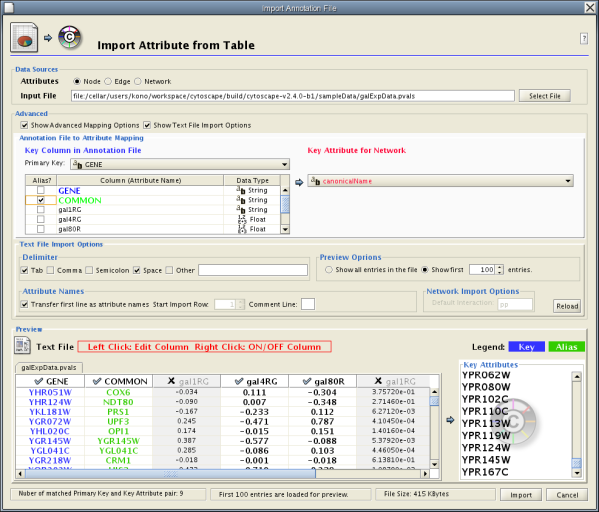
\includegraphics[scale=1]{images/attribute_table_import_main.png} 

 \emph{\textbf{Sample Attribute Table 1} }

 \textbf{Table\^A 12.\^A }

\begin{tabular}{|c|c|c|c|}
\hline 
 & & & \\
\hline 

 Object Key


 Alias


 SGD ID
 &

 AAC3


 YBR085W|ANC3


 S000000289
 &

 AAT2


 YLR027C|ASP5


 S000004017
 &

 BIK1


 YCL029C|ARM5|PAC14


 S000000534
 \\
 \hline 

\end{tabular}

 The attribute table file should contain a primary key column and at least one attribute column. The maximum number of attribute columns is unlimited. The \emph{Alias}
 column is an optional feature, as is using the first row of data as attribute names. Alternatively, you can specify each attribute name from the File \^a†’ Import \^a†’ Attribute from Table (text/MS Excel)... user interface. 


 \textbf{Basic Operation}


 The user interface of the ``Import Attributes from Table'' window is similar to that of the ``Import Network from Table'' window. 
\begin{enumerate}
\item 

 Select File \^a†’ Import \^a†’ Attribute from Table (text/MS Excel)... 

\item Select one of the attribute types from the Attributes radio buttons. Cytoscape can import node, edge, and network attributes. 
\item Select a data file. To load a local file, click on the Select File button and choose a data file. This can be either a text or Excel (.xls) file. To load a remote file, type the source URL directly into the text box. To show a preview of the remote file, click the Reload button on the Show Text File Import Options panel. 
\item (Optional) If the table is not properly delimited in the preview panel, change the delimiter in the Text File Import Options panel. The default delimiter is the tab. This step is not necessary for Excel Workbooks. 
\item By default, the first column is designated as the primary key. Change the key column if necessary. \begin{itemize}
\item 

 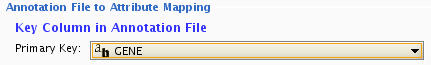
\includegraphics[width=\textwidth]{images/attribute_table_import_primary_key.png} 


\end{itemize}

\item Click the Import button. 

\end{enumerate}


 
\textbf{Advanced Options}


 \textbf{Mapping Key Attributes to the primary key}


 Formerly, Cytoscape only supported mapping between node/edge IDs and the primary keys in attribute files. With the introduction of Cytoscape 2.4, this limitation has been removed, and now both IDs and attributes with primitive data types (string, boolean, floating point, and integer) can be selected as the Key Attribute using the dropdown list provided. Complex attributes such as lists are not supported. 


 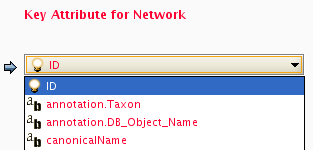
\includegraphics[width=\textwidth]{images/attribute_table_import_keyattr.png} 


 
\textbf{Aliases}


 Cytoscape uses a simple mechanism to manage aliases of objects. Both nodes and edges can have aliases. If an attribute is loaded as an alias, it is treated as a special attribute called ``alias''. This will be used when mapping attributes. If the primary key and key attribute for an object do not match, Cytoscape will search for a match between aliases and the key attribute. To define an alias column in the attribute table, just click on the checkboxes to the left of the column name while importing. 


 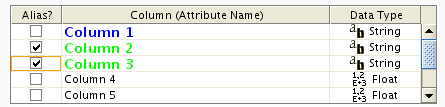
\includegraphics[width=\textwidth]{images/attribute_table_import_alias.png} 


 
\textbf{Text File Import Options}


 For more detail on these options, please see the ``Import Free-Format Table Files'' section of the user manual in the Creating Networks chapter. 


 

\textbf{Attribute Browser}


 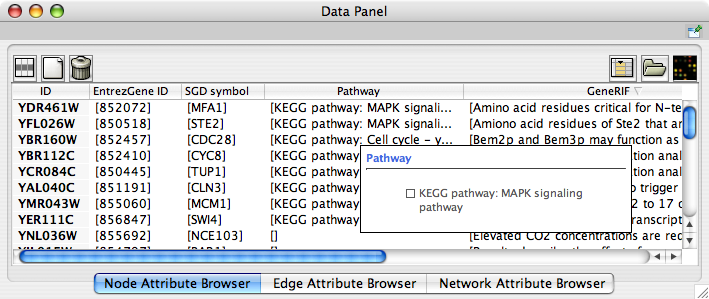
\includegraphics[width=\textwidth]{images/attribute_browser26.png} 


 When Cytoscape is started, the Attribute Browser appears in the bottom CytoPanel. This browser can be hidden and restored using the F5 key or the View \^a†’ Show/Hide attribute browser menu option. Like other CytoPanels, the browser can be undocked by pressing the little icon in the browser\^a€™s top right corner. 


 To swap between displaying node, edge, and network attributes use the tabs on the bottom of the panel labelled ``Node Attribute Browser'', ``Edge Attribute Browser'', and ``Network Attribute Browser''. The attribute browser displays attributes belonging to selected nodes and/or edges and the currently selected network. To populate the browser with rows (as pictured above), simply select nodes and/or edges in a loaded network. By default, only the ID of nodes and edges is shown. To display more than just the ID, click the Select Attributes 
\includegraphics[scale=1]{images/attributes_select_icon.png}  button and choose the attributes that are to be displayed (select various attributes by clicking on them, and then click elsewhere on the screen to close the attribute list). Each attribute chosen will result in one column in the attribute browser. Most attribute values can be edited by double-clicking an attribute cell; list values cannot be edited, and neither can the ID. Attribute rows in the browser can be sorted alphabetically by specific attribute by clicking on a column heading. A new attribute can be created using the Create New Attribute 
\includegraphics[scale=1]{images/attributes_new_icon.png}  button, and must be one of four types \^a€“ integer, string, real number (floating point), or boolean. Attributes can be deleted using the Delete Attributes 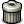
\includegraphics[scale=1]{images/attributes_delete_icon.png}  button. \textbf{NOTE: Deleting attributes removes them from Cytoscape, not just the attribute browser!}
 To remove attributes from the browser without deleting them, simply unselect the attribute using the Select Attributes 
\includegraphics[scale=1]{images/attributes_select_icon.png}  button. 


 The right-click menu on the Attribute Browser has several functions, such as exporting attribute information to spreadsheet applications. For example, use the right-click menu to Select All and then Copy the data, and then paste it into a spreadsheet application. Each attribute browser panel also has a button for importing new attributes: 
\includegraphics[scale=1]{images/attributes_import_icon.png}  . 


 The Node Attribute Browser panel has additional buttons for loading Gene Expression attribute matrices ( 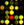
\includegraphics[width=1em]{images/attributes_gene_expr_icon.png}  ) as node attributes. 


 \textbf{Attribute Batch Editor}


 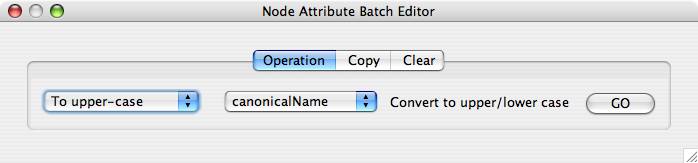
\includegraphics[width=\textwidth]{images/attribute_editor26.png} 


 From Cytoscape 2.6, Attribute Browser has new \textbf{Attribute Batch Editor}
. This enables you to set and modify attribute values at once. This function changes values for selected nodes or edges. For example, if you want to create a new attribute called \emph{Modules}
 and set module names for each group of selected nodes, you can use \emph{Set}
 command from this editor. 
